\chapter{The SMELLIE Calibration System}\label{chap:smellie_hardware}
\epigraph{\textit{There's a certain Slant of light,\\
Winter Afternoons ---\\
That oppresses, like the Heft\\
Of Cathedral Tunes ---}}{\textsc{Emily Dickinson}}

As mentioned in Section~\ref{sec:eo_calibs}, one of the principal systems for calibrating the optics of the SNO+ detector is SMELLIE. This calibration device consists of 5 different optical wavelength lasers able to be fired through 15 optical fibres, whose endpoints are attached to the PSUP. A collimator is attached at the end of each fibre, ensuring the emitted light forms a narrow beam across the detector. A diagram of SMELLIE in the detector is shown in Fig.~\ref{fig:smellie_diagram}.

\begin{figure}
    \centering
    % \includegraphics[]{}
    \caption[]{}
    \label{fig:smellie_diagram}
\end{figure}

The primary goal of SMELLIE is the measurement and monitoring of optical scattering within the detector over the lifetime of the experiment. By firing light from SMELLIE into the detector, some fraction of the photons will be scattered by the detector medium, a fraction of those scattering at large angles relative to the direction of the SMELLIE beam. This strongly scattered light can be detected by PMTs far from the `beamspot', and will also arrive substantially later than light which travelled directly from the fibre to those PMTs. By isolating this scattered light signal, and comparing the quantity observed in data to equivalent simulations with varying scattering lengths, in principle one can measure the detector medium's scattering length. If one takes SMELLIE data with various wavelengths of light at various points in time, we can get a dynamical picture of the optical scattering in SNO+. An analysis of optical scattering in the scintillator phase is made in Section~\ref{sec:scattering_analysis}.

Another substantial measurement that can be made with SMELLIE is the extinction length of the detection media as a function of wavelength and time. This can be done by comparing the fraction of light emitted by the fibre that gets observed in the beamspot after passing through the detector. Section~\ref{sec:ext_length_analysis} covers this analysis in the scintillator phase. Once measurements of both the scattering length and extinction length have been made, it is then possible to derive the absorption length from Eq.~\ref{eq:ext_length_def}.

Why is measuring the scattering and absorption lengths of the detector medium important? Both optical characteristics of the detector impact the propagation of light from physics events, and hence which PMTs get hit along with the times of those hits. If these lengths are systematically off within simulation, this can lead to negative consequences for reconstructing events. In particular, for the scintillator phase, if there is more optical absorption occurring than expected, then because not all absorbed light is re-emitted a larger fraction of photons are lost. Therefore, because energy reconstruction is strongly dependent on the number of PMT hits observed in an event, the energy of events will be systematically under-estimated. Alongside this, light that is re-emitted will only do so after some time delay, and the direction of this re-emission unlikely to be in the same direction as before. This leads to systematic changes in the observed time residual distributions, impacting position reconstruction, as well as any classifiers that use the time residual distribution.

If there is more optical scattering than expected within the scintillator, this also indirectly leads to a greater loss of light because of the increased path length that a photon will typically have to travel before being detected. By consequence, there will be a second-order impact on the energy reconstruction from systematics in the scattering length. Much like changes in the quantity of re-emitted light, increasing the amount of scattering will also systematically effect the position reconstruction and many classifiers.

This chapter covers the hardware used to take SMELLIE data, as well as the steps taken to ensure high quality data was taken throughout the scintillator phase of the experiment.

% \begin{itemize}
%     \item Basic principle for how SMELLIE works: firing collimated laser light into detector to observe scattering events.
%     \item Analysis will measure and monitor scattering in a detector with changing optics.
%     \item One can try and measure some component of this: the cross-section/scattering length versus wavelength and time, and/or the relative scattering length versus wavelength and time.
% \end{itemize}
% [1 page]

\section{The SMELLIE Hardware}\label{sec:smellie_hardware}
A full description of the initial hardware setup that was used during the air fill and early parts of the water fill phase can be read in~\cite{}. % cite Krish & DocDB #3511
Since then, a series of hardware upgrades have been made, with~\cite{} % cite Esther (+more?)
covering the hardware status used in data taken throughout the water phase.
Fig.~\ref{fig:smellie_timeline} shows a timeline of the hardware upgrades as well as the data taking campaigns performed throughout the current lifetime of the experiment. The current layout of the SMELLIE hardware, showing the connections between each of the devices within the system, can be seen in Fig.~\ref{fig:smellie_diagram_detailed}. The rest of this section briefly summarises the current contents of the calibration system, along with descriptions of the major hardware changes made since the water phase.

\begin{figure}
    \centering
    % \includegraphics[]{}
    \caption[]{}
    \label{fig:smellie_timeline}
\end{figure}

\begin{figure}
    \centering
    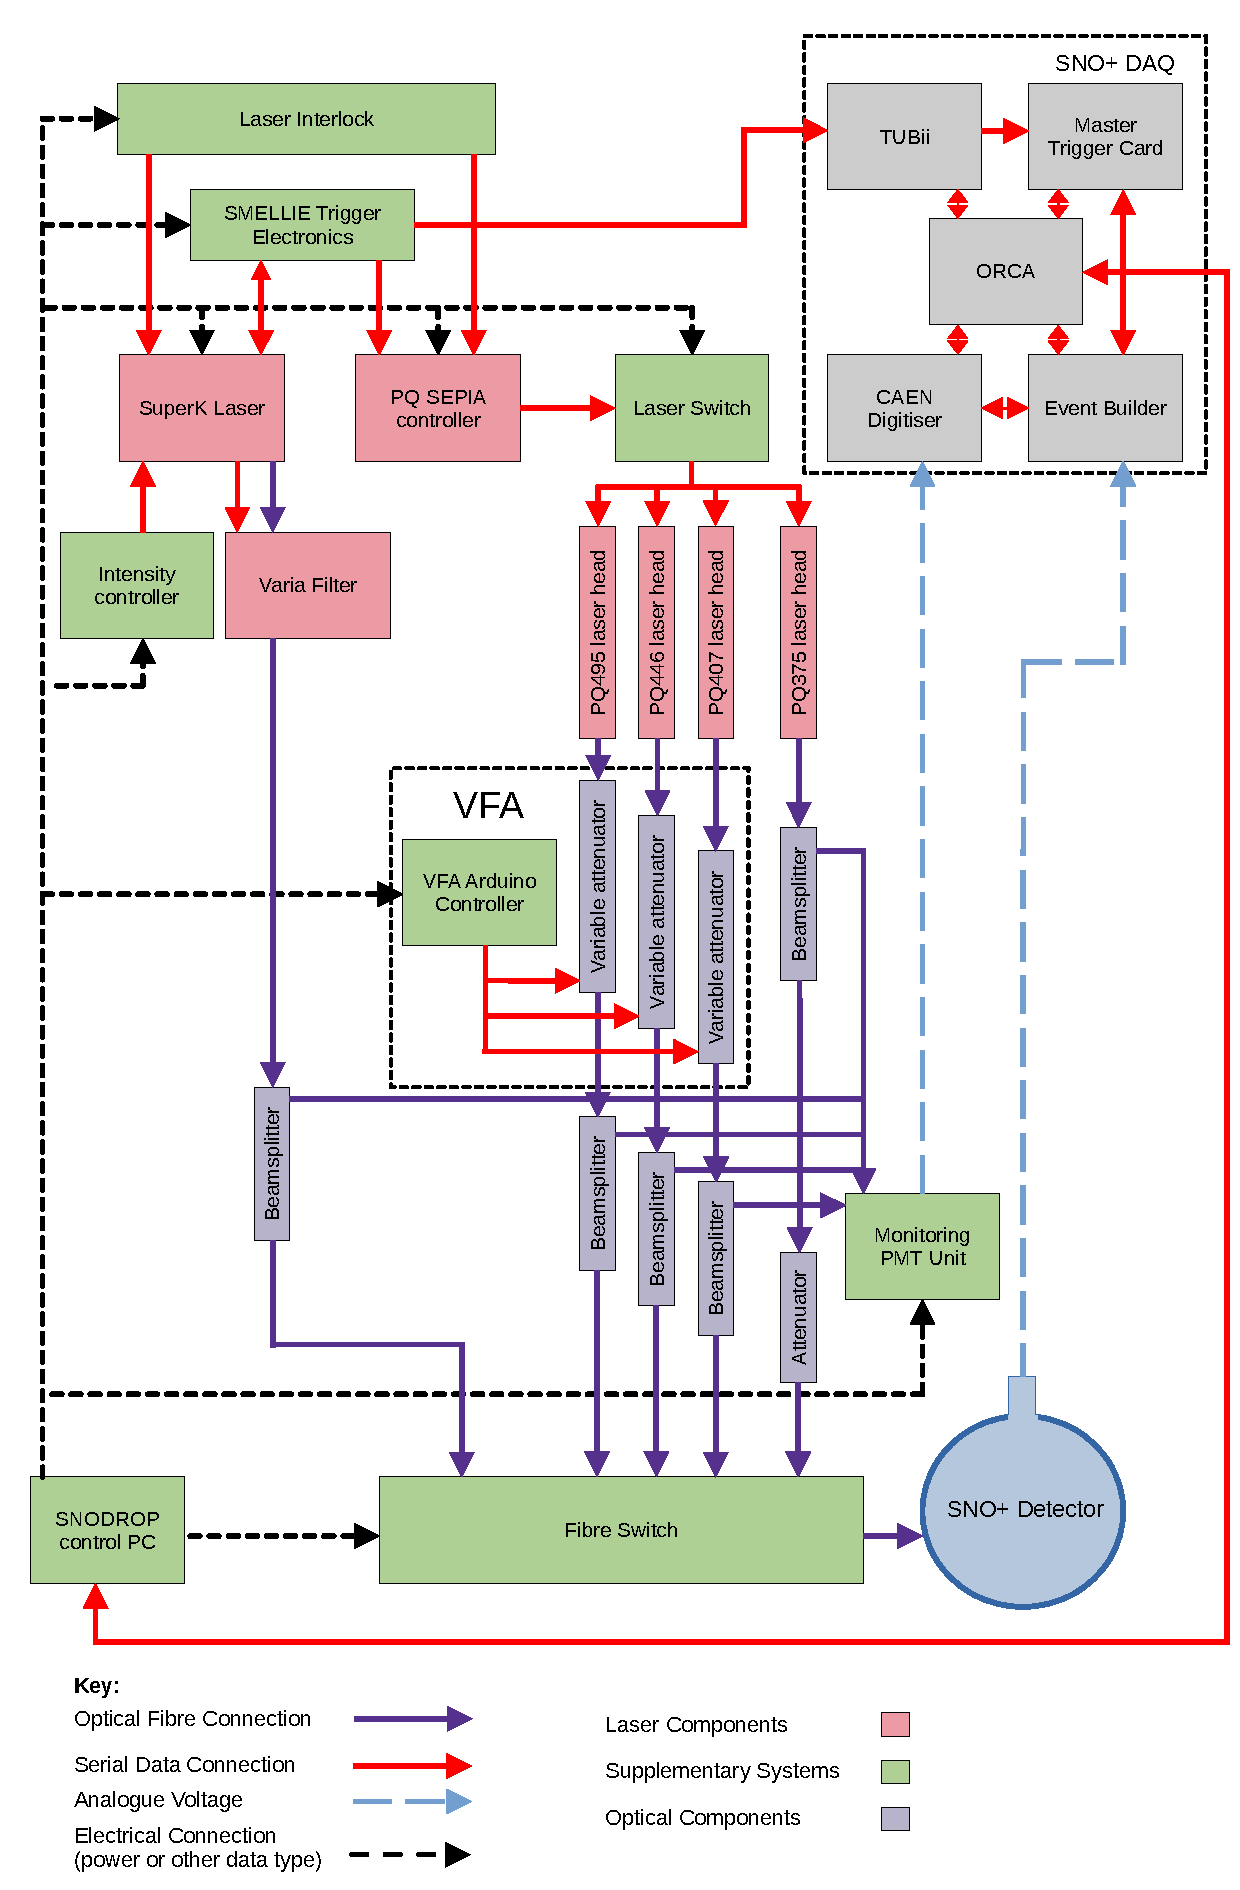
\includegraphics[width=0.95\linewidth]{3_SMELLIEHardware/images/smellie_hardware_schematic.pdf}
    \caption[Diagram of the connections between the various bits of SMELLIE hardware and the rest of the SNO+ detector]
    {Diagram of the connections between the various bits of SMELLIE hardware and the rest of the SNO+ detector, after the changes made in the Summer of 2022. Adapted from~\cite{turnerMeasurementScatteringCharacteristics2022}.}
    \label{fig:smellie_diagram_detailed}
\end{figure}

\subsection{Lasers}\label{sec:smellie_lasers}
\nomenclature{\textbf{PQ}}{PicoQuant}
Fundamental to the SMELLIE calibration system are 5 optical-wavelength lasers. Four of these are fixed-wavelength pulsed-diode laser heads from the company PicoQuant. These `PQ' laser heads each emit with a different narrow wavelength spectrum, peaking at \SI{375}{\nm}, \SI{407}{\nm}, \SI{446}{\nm}, and \SI{495}{\nm}. These are referred to as the PQ375, PQ407, PQ446, and PQ495 lasers, respectively. In addition to these lasers, a SuperK Compact laser made by NKT Photonics (hereafter referred to as the SuperK laser) is also used\footnote{
    Apologies to those more familiar with `SuperK' referring to the SuperKamiokande experiment based in Japan: this laser bears no relation.
}. Unlike the PQ laser heads, the SuperK is a super-continuum laser able to produce laser light over the whole optical wavelength spectrum. Because we are almost always interested in determining optical properties at specific wavelengths, a variable bandpass filter also built by NKT Photonics known as the SuperK Varia has been included. This allows the user to select any wavelength interval between \SIrange{400}{700}{\nm}, with a minimum bandwidth of \SI{10}{\nm}. The wavelength and emission timing characteristics of all five lasers are shown in Fig.~\ref{fig:smellie_emission_wav_timing}. The $\mathcal{O}(\SI{1}{\ns})$ time widths for the lasers are essential for scattering analyses as they allow for much greater precision in knowing when photons should arrive at PMTs in the detector than with an LED source. This is why SMELLIE uses lasers for its light generation, unlike the LEDs used for AMELLIE and TELLIE.

\begin{figure}
    \centering
    \begin{subfigure}{0.98\textwidth}
        \centering
        % 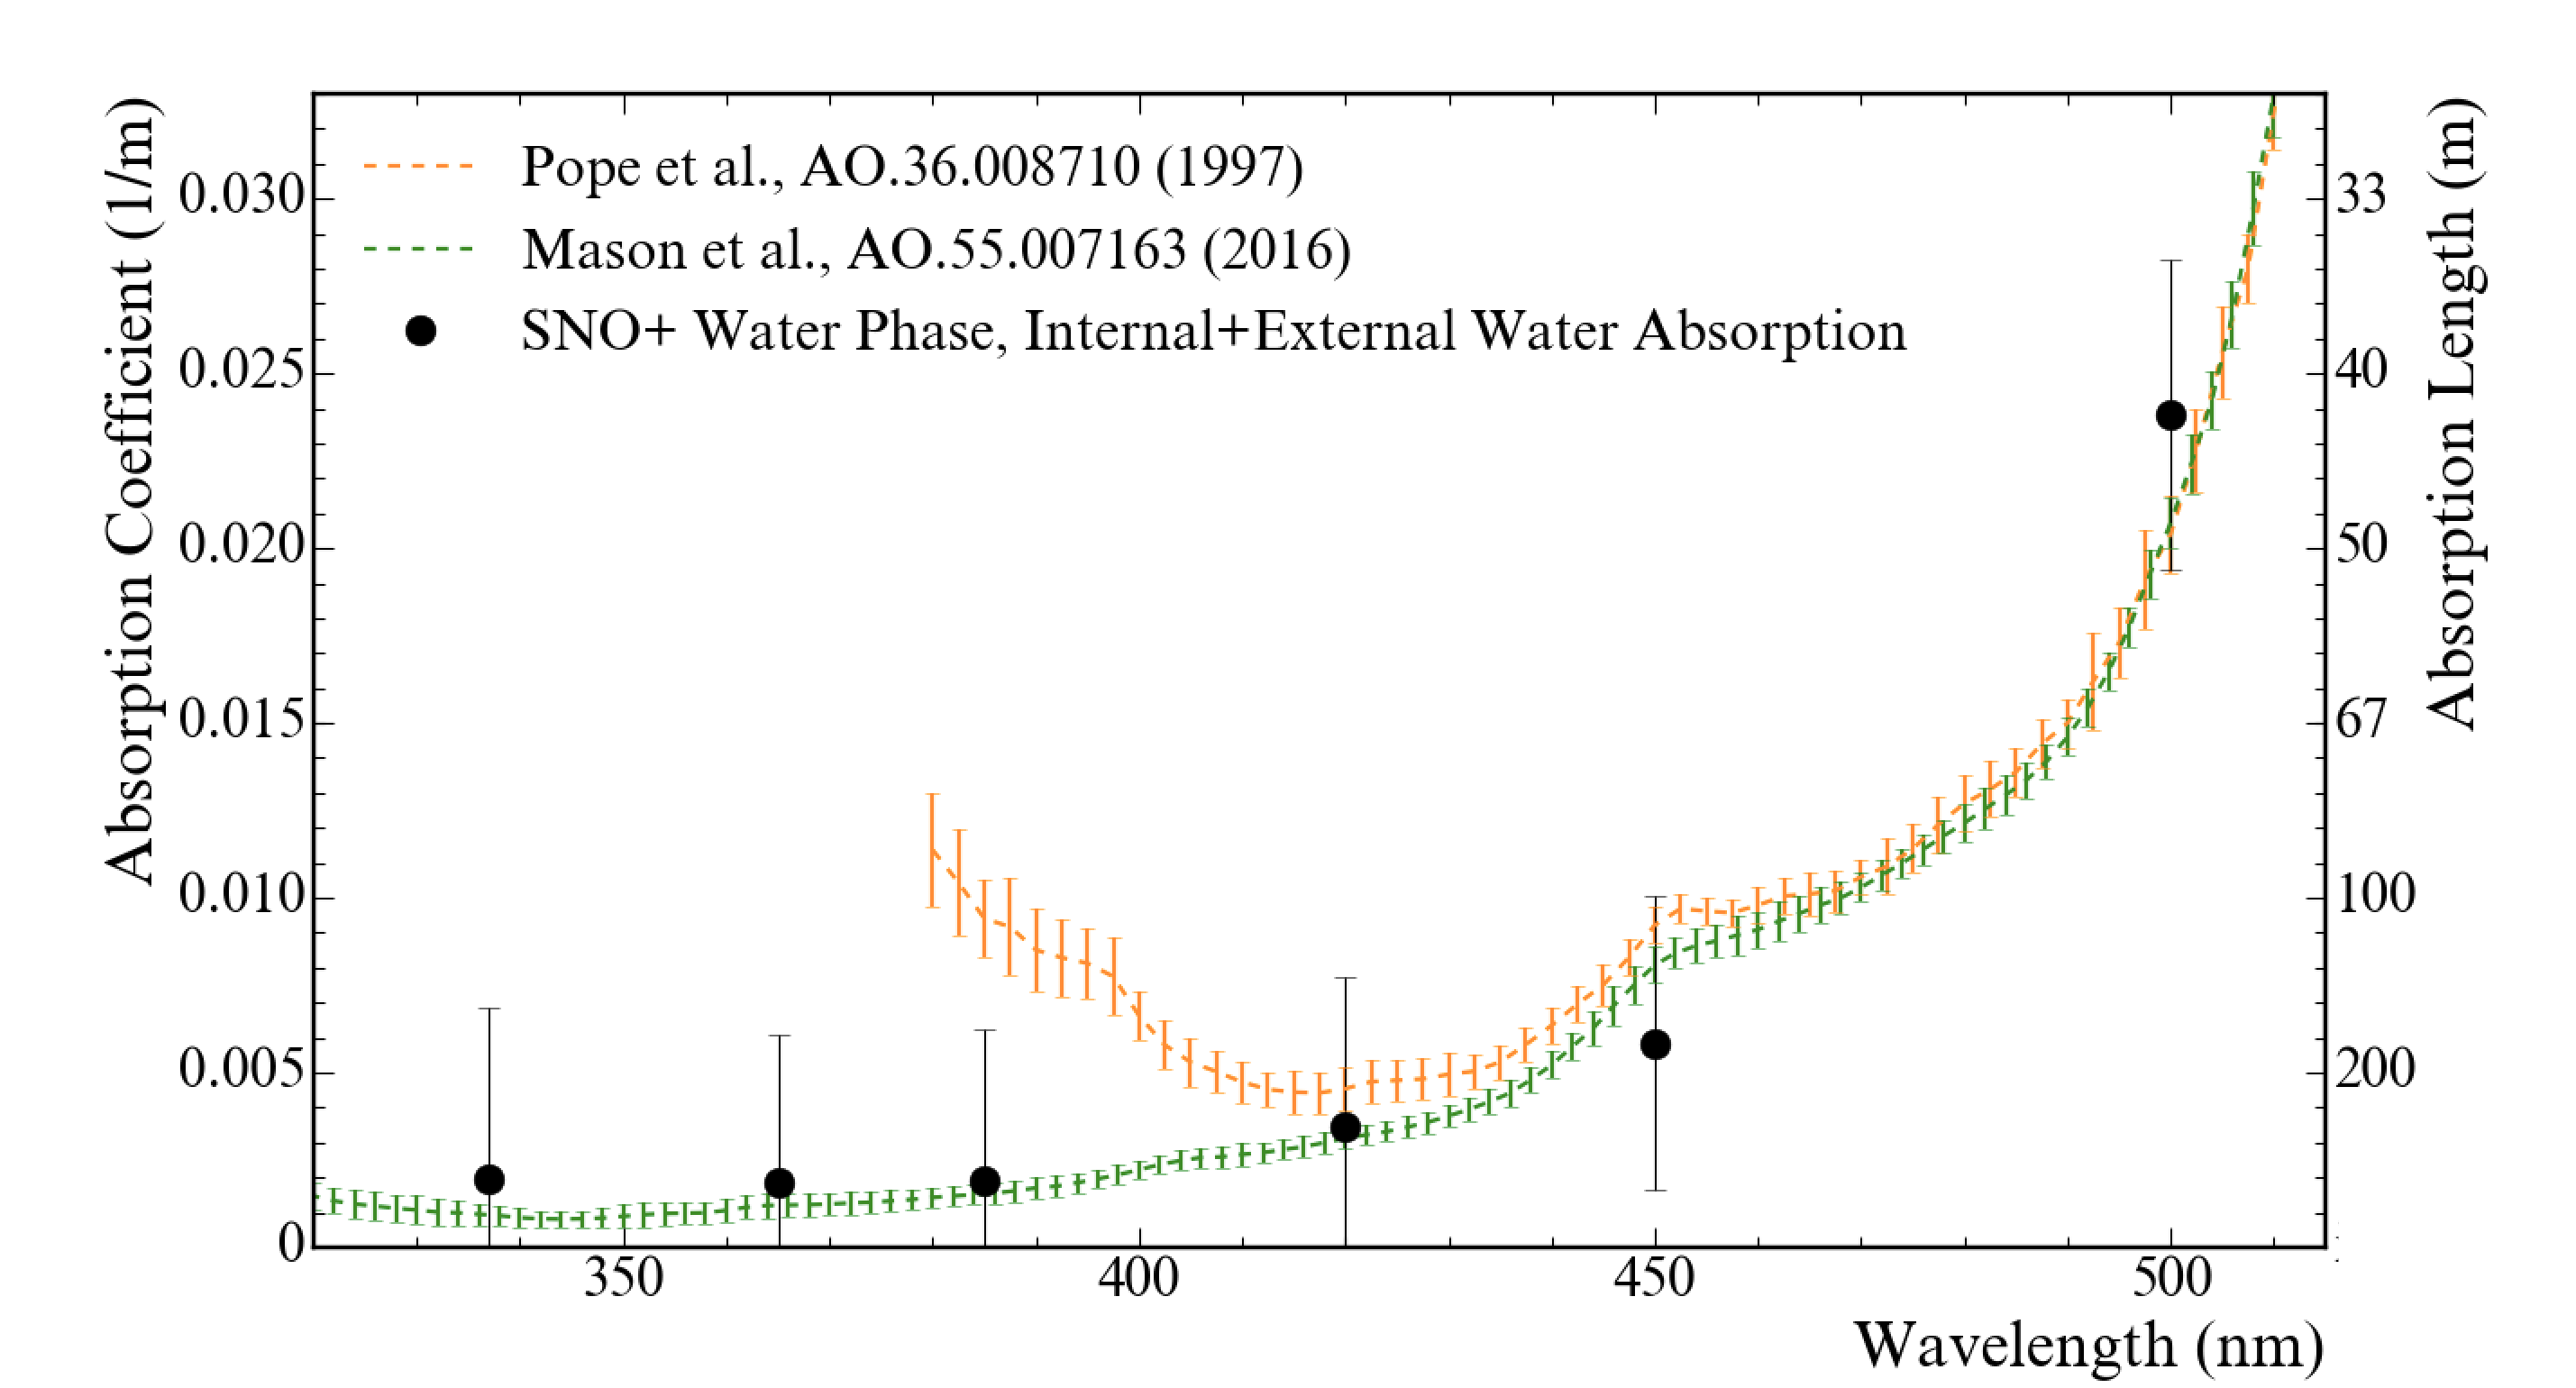
\includegraphics[width=0.9\textwidth]{2_Detector/Figs/WaterAbsorption.png}
        \caption{}
        \label{fig:smellie_emission_wavelengths}
    \end{subfigure}
    \begin{subfigure}{0.98\textwidth}
        \centering
        % 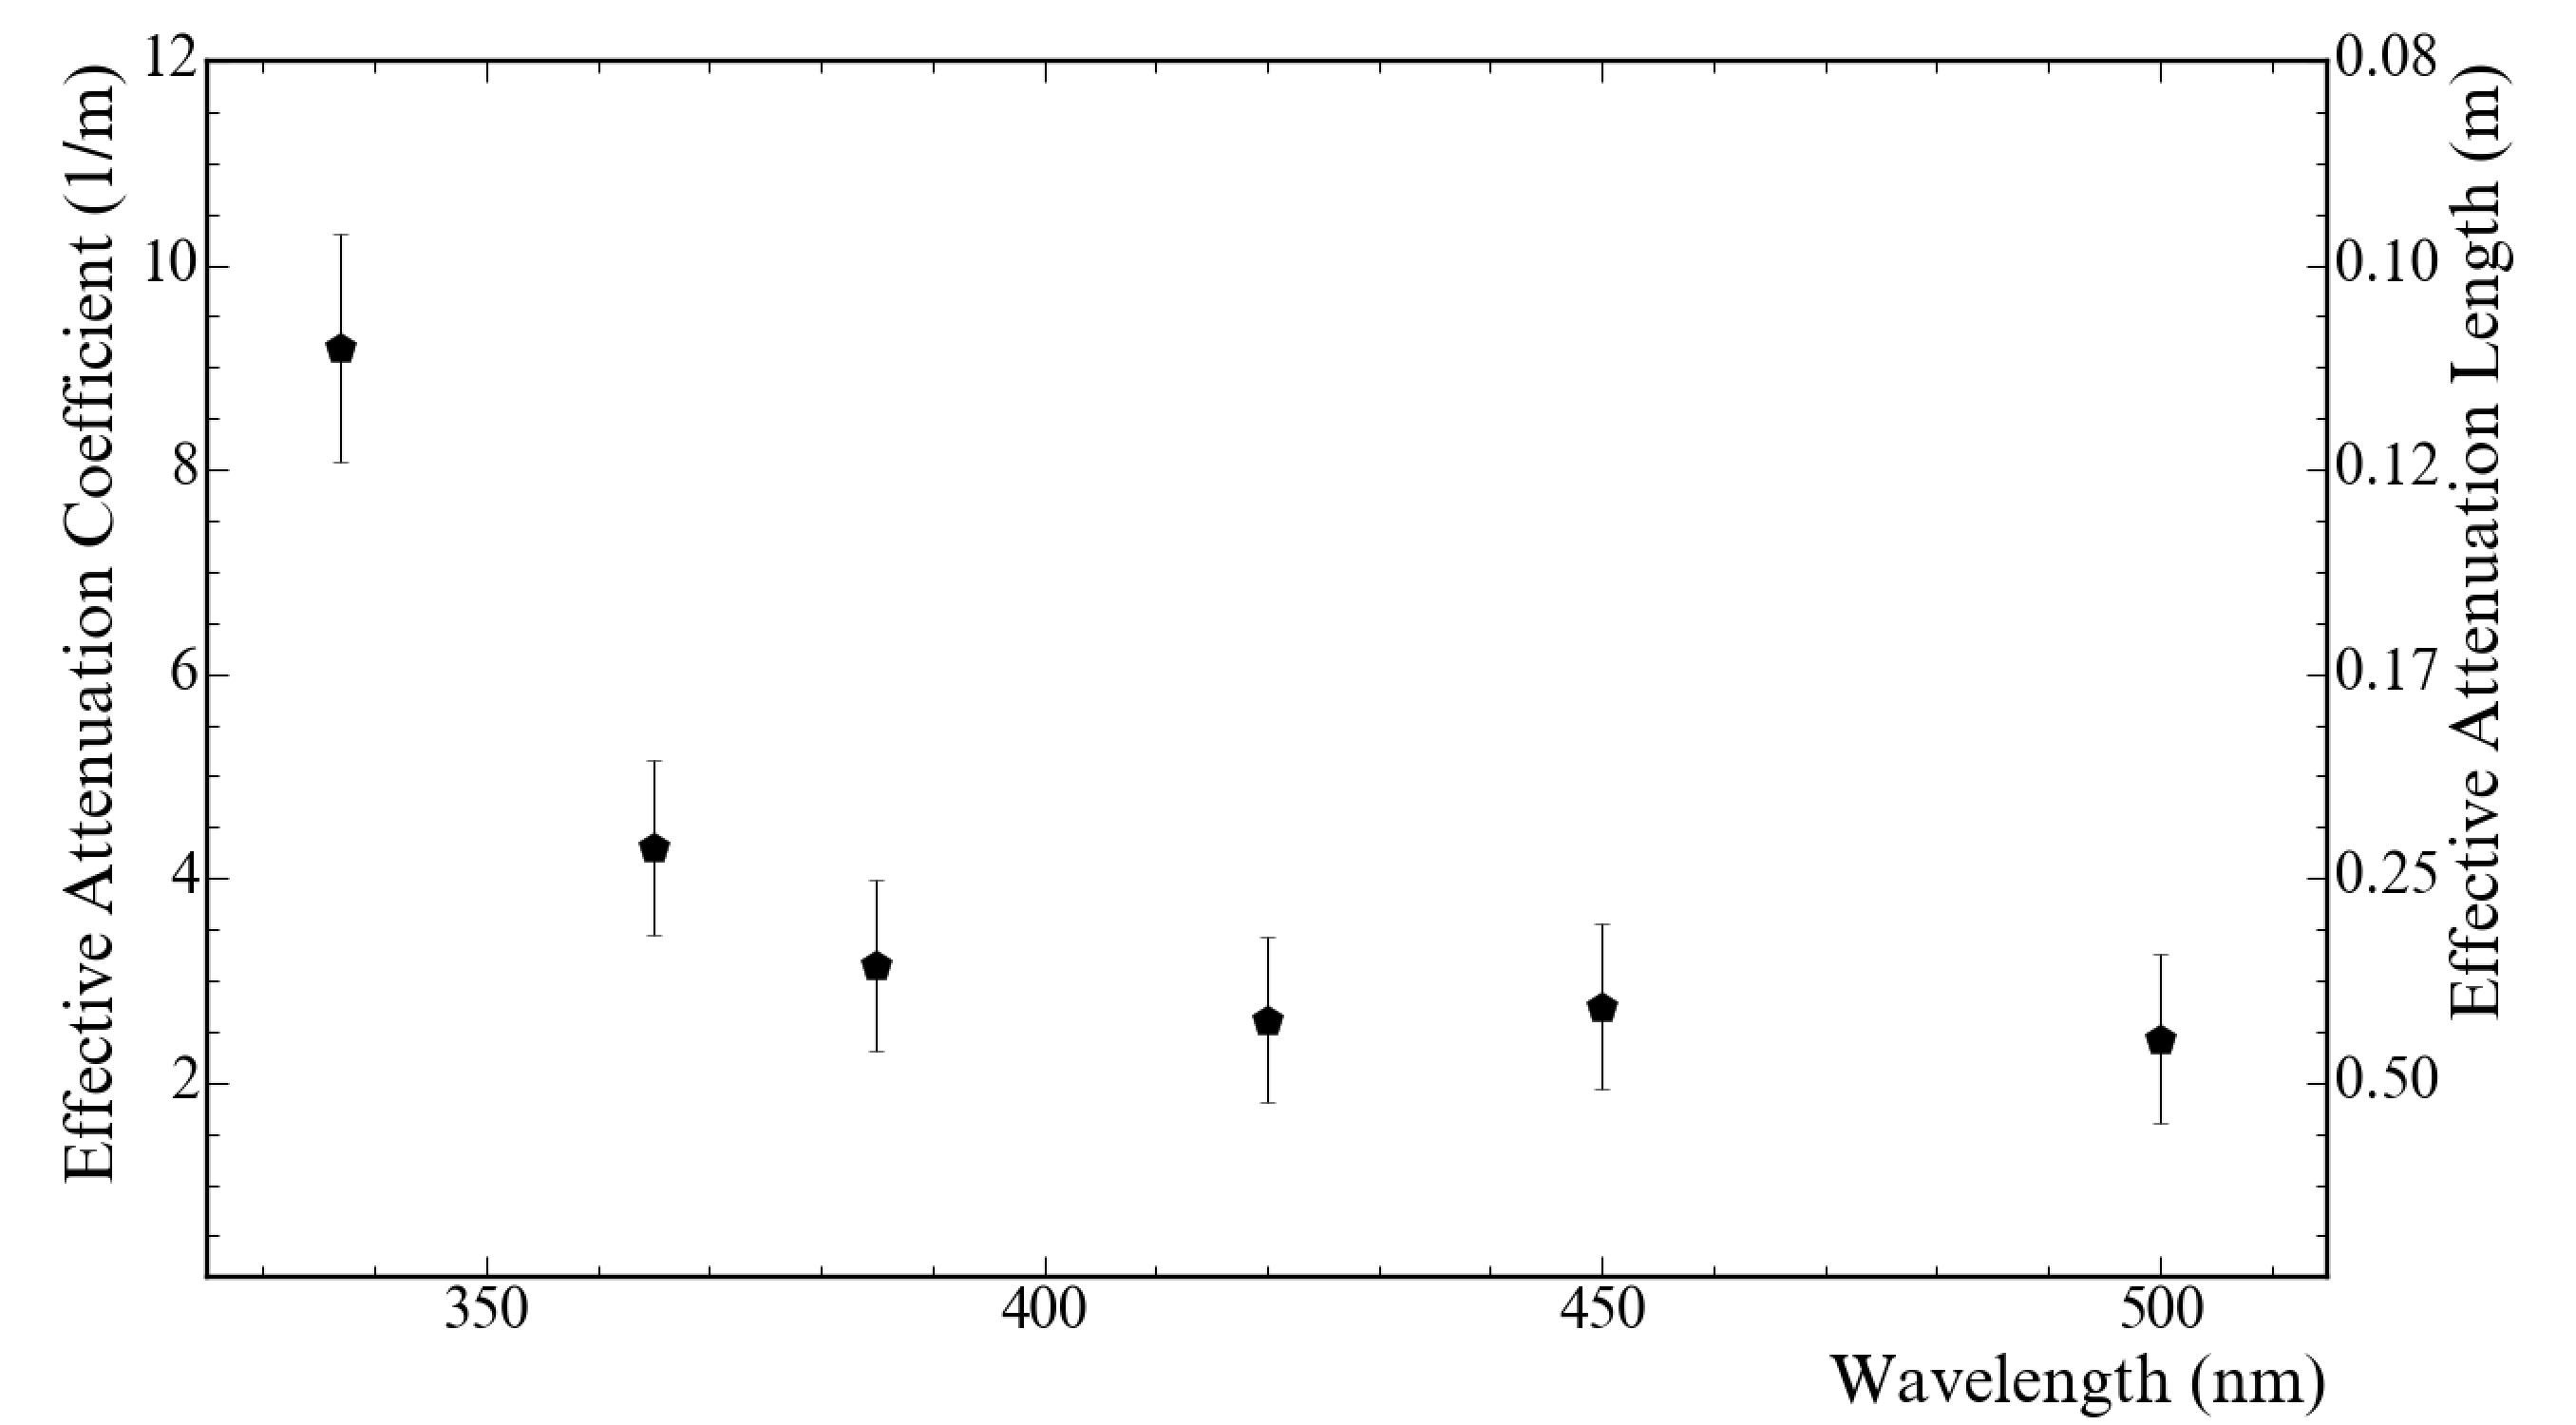
\includegraphics[width=0.85\textwidth]{2_Detector/Figs/AcrylicAttenuation.png}
        \caption{}
        \label{fig:smellie_emission_timing}
    \end{subfigure}
    \caption{}
    \label{fig:smellie_emission_wav_timing}
\end{figure}

\subsection{Controlling Laser Intensities}\label{sec:smellie_attenuators}
It is important to be able to control the quantity of light that enters the detector from a given pulse of one of the lasers. Too much light, and because of the detector's DAQ analysis of data becomes difficult, and in the extreme case permanent damage could be done. Too little, and insufficient statistics are collected by the detector to actually do any analysis. Controlling the pulse intensity of light into the detector is done in two parts. For the SuperK laser, the raw power of the beam in a pulse can be set as a percentage of the maximum possible power for that wavelength. Once a light pulse has been generated, it is then attenuated by a neutral density filter contained within the SuperK laser hardware.

For the PQ lasers, a PicoQuant-brand SEPIA II laser driver is used to set the raw pulse intensity and firing rate. Unlike the SuperK, the intensity control is given by the laser driver's driving voltage, as a fraction of the maximum possible voltage. Problematically, the dependence on the raw output intensity of the PQ laser heads are highly nonlinear with respect to the amplitude of the driving voltage. To demonstrate, consider the observed npe per shot within the detector as a function of driving voltage for SMELLIE events using the PQ lasers: see Fig.~\ref{fig:pq_old_intensity_dependence}. For low driving voltages, the resulting npe is very small, and rises slowly. However, near a certain `lasing threshold' the npe observed increases super-exponentially, rapidly climbing many orders of magnitude in intensity. Above this threshold, increasing the driving voltage once again changes the observed intensity relatively slowly. A result of this is that if one requires an npe in the detector associated with a driving voltage that lies near the threshold, then any uncertainty in that driving voltage value can lead to dramatic changes in the npe observed. Furthermore, when driving a laser head near its lasing threshold the shot-to-shot variation in intensity can also become substantial: see Fig.~\ref{fig:pq_threshold_intensity_variation} for an example of this occurring.

\begin{figure}
    \centering
    % \includegraphics[]{}
    \caption[]{}
    \label{fig:pq_old_intensity_dependence}
\end{figure}

\begin{figure}
    \centering
    % \includegraphics[]{}
    \caption[]{}
    \label{fig:pq_threshold_intensity_variation}
\end{figure}

During the water phase and for much of the scintillator phase, much of the data taken, especially using the PQ407 and PQ446 lasers, suffered from large shot-to-shot intensity variations. Throughout this period, after the light was generated by a PQ laser head it would then be passed through an attenuator, fixed to some nominal attenuation setting for each laser. In theory, one could solve the intensity variation problem by deliberately setting the intensity well beyond the lasing threshold, and then changing the attenuation of the attenuator to obtain the npe within the detector one is interested in. However, under the original hardware this was untenable as this would require someone to manually change the attenuations in-person every time a different set of SMELLIE run conditions were proposed.

\nomenclature{\textbf{VFA}}{Remotely-controllable Variable Fibre Attenuator}
Instead, Jeff Lidgard built a piece of hardware called the remotely-controllable Variable Fibre Attenuator (VFA), shown in Fig.~\ref{fig:vfa_picture}. Contained within a metal housing were a `precision variable attenuator' from DiCon Fibreoptics~\cite{} % cite DiCon attenuator specsheet online
for each PQ laser, along with an Arduino running firmware written by Jeff to enable communication with each of the attenuators. Commands could be sent to a given attenuator asking for a specific attenuation between \SIrange{0}{3000}{\dB}.
Following ex-situ testing by Jeff Lidgard and Jasmine Simms, the VFA was installed underground by myself and Armin Reichold in July 2022, with some assistance from Jeff in integration of the hardware and SMELLIE server software.

\begin{figure}
    \centering
    % \includegraphics[]{}
    \caption[]{}
    \label{fig:vfa_picture}
\end{figure}

During testing of the VFA in-situ, it was discovered that the inherent attenuation of the variable attenuator at the minimum setting of \SI{0}{\dB} for the PQ375 laser was so strong that negligible light was ever observed in the detector. Because of this, the PQ375 was not hooked up to the VFA, and kept its original attenuator setup. After fixing the driving voltage settings for PQ407, PQ446, and PQ495 to be XXX, XXX, and XXX respectively, % add in numbers!
the observed npe in the detector was once again compared to the input intensity setting. For PQ375 this input parameter remained the driving voltage; for the others, the attenuation setting was now used. The results can be seen in Fig~\ref{fig:pq_new_intensity_dependence}. As hoped for, the three PQ lasers hooked up to the VFA can now have stable intensities of light observed in the detector over multiple orders of magnitude of observed intensity.

\begin{figure}
    \centering
    % \includegraphics[]{}
    \caption[]{}
    \label{fig:pq_new_intensity_dependence}
\end{figure}

\subsection{Propagation of Light into the Detector}\label{sec:smellie_fibres}
Once a pulse of optical light has been generated by the lasers and attenuated to the desired intensity, the next step is to navigate that light into the detector. This is achieved through a network of Corning-brand ``InfiniCor SXi'' multimode optical fibres~\cite{}. % cite Corning datasheet(s)
These fibres were chosen in part for their low intrinsic radioactivity~\cite{}, % cite Radon Assay/Krish's thesis
as well as having a graded index as a function of radius. This latter property enables lower dispersion between different modes of the light, so that the initial sharpness of any given light pulse in time is maintained. However, because these fibres were mainly designed for telecommunication purposes, their nominal operating wavelengths are out in the near-infrared, \SIrange{750}{1450}{\nm}. As SMELLIE only fires wavelengths in the range \SIrange{375}{700}{\nm}, there is a small but non-negligible amount of light lost when propagating through the fibres.

After some light is split off by a beamsplitter to allow for ex-situ monitoring of the light pulse (see Section~\ref{sec:smellie_mpu}), it is sent to the Fibre Switch, two boxes manufactured by Laser Components UK~\cite{} % cite Laser Components UK
that allows a user to remotely-control which of the fibres to send the light down into the detector.

Finally, the light that passes through the fibre switch propagates along one of the 15 optical fibres that have been submerged in the SNO+ cavity, whose ends are mounted to the PSUP. Specifically, sets of three fibres are mounted to a given node of the PSUP, with associated node numberings: nominally 07, 25, 37, 55, and 21. These provide for a variety of positions within the detector from which light can be emitted. Each mounting which holds three of the optical fibres also contains collimators, designed to reduce the possible range of angles with which the light can be emitted from. This is particularly important for SMELLIE, because unlike the other ELLIE systems, a thin `pencil' beam of light across the detector is ideal for measuring scattering~\cite{majumdarMeasurementOpticalScattering2015}. % cite Krish.
One last thing the mounting achieves is to point each of the three fibres in different directions: \ang{0}, \ang{10}, and \ang{20} from the direction radially towards the centre of the detector.

Each fibre is given a name that nominally refers to both its mounting position and its pointing direction. For example, the label `FS107' corresponds to the SMELLIE fibre mounted at node 07 with a pointing direction of \ang{10}. Unfortunately, during installation some fibres were mislabelled, leading to the node mounting points and pointing directions of some fibres being inconsistent with the labelling convention. The actual pointing directions for each fibre can be seen in Table~\ref{tab:smellie_fibre_labellings}.
The 3D positions and pointing directions of all the fibres are shown in Fig.~\ref{fig:smellie_pos_dirs}.

\begin{table}
    \centering
    \begin{tabular}{c c c}
        \hline
        Fibre   & Node & Pointing direction \\ \hline \hline
        FS007   & 07   & \ang{0}  \\
        FS107   & 07   & \ang{10} \\
        FS207   & 07   & \ang{20} \\
        FS025   & 25   & \ang{0}  \\
        FS125   & 25   & \ang{10} \\
        FS225   & 25   & \ang{20} \\
        FS037   & 37   & \ang{10} \\
        FS137   & 37   & \ang{0}  \\
        FS237   & 37   & \ang{20} \\
        FS055   & 55   & \ang{10} \\
        FS155   & 55   & \ang{20} \\
        FS255   & 55   & \ang{0}  \\
        FS093   & 21   & \ang{0}  \\
        FS193   & 21   & \ang{10} \\
        FS293   & 21   & \ang{20} \\
        \hline
    \end{tabular}
    \caption[SMELLIE fibre names, their associated mounting nodes on the PSUP, and their pointing direction.]
    {SMELLIE fibre names, their associated mounting nodes on the PSUP, and their pointing direction. Taken from~\cite{turnerMeasurementScatteringCharacteristics2022}.}
    \label{tab:smellie_fibre_labellings}
\end{table}

\begin{figure}
    \centering
    % \includegraphics[]{}
    \caption[]{}
    \label{fig:smellie_pos_dirs}
\end{figure}

\subsection{The Monitoring PMT Unit}\label{sec:smellie_mpu}
\nomenclature{\textbf{MPU}}{Monitoring PMT Unit (for SMELLIE)}
As mentioned in the previous section, part of the light generated by the lasers gets split off from the main fibre path down into the detector, and instead is used for monitoring purposes. This is achieved with a box known as the Monitoring PMT Unit (MPU). As the name suggests, the MPU contains a small PMT that generates an electronic signal pulse from the laser light. This signal is then shaped by electronics, and passed to the detector's central CAEN digitiser to have that pulse digitised.

One problem with the existing MPU within SMELLIE was that the pulse it produced was so broad that 300 ADC samples were needed to capture the full shape (the CAEN samples at a rate of 1 every \SI{4}{\ns}). This led to a large fraction of data being generated by SMELLIE events coming not from the PMT hit information, but simply the MPU's signal digitisation. A natural consequence of this was the rate at which the lasers could be fired had to be limited to typically \SI{1}{\kHz}, otherwise the detector was not able to handle the rate of data being generated.

Because of this, a new MPU was commissioned. Built by Adam Baird and Johan Fopma from the Oxford Physics Central Electronics Group, this MPU had updated electronics such that the pulse was shaped shorter. In addition, the rise time of the pulse was made faster, in the hopes that the emission time of the light pulse for a given event could be captured more accurately. The new MPU was installed by myself and Armin Reichold at the same time as the VFA, in Summer 2022.

Alongside the installation of the new hardware, the settings in ORCA for the CAEN digitisation of the MPU signal were updated. In particular, the number of samples made by the CAEN was shortened from 300 down to 124. The timing of the CAEN sampling and delay on the TUBii trigger (more on the trigger shortly) was also modified. As a result of these changes, the shortest possible trace was now being generated, without missing any part of the MPU pulse or moving the observed TAC for hits in the detector outside the trigger window. Fig.~\ref{fig:caen_trace_comparison} shows a comparison between typical MPU pulses taken before and after the upgrades.

\begin{figure}
    \centering
    % \includegraphics[]{}
    \caption[]{}
    \label{fig:caen_trace_comparison}
\end{figure}

\subsection{Event Triggering and Data Acquisition}\label{sec:smellie_triggering_daq}
As mentioned in Section~\ref{sec:daq}, it is possible to trigger the SNO+ detector electronics via an external asynchronous trigger, EXTA. Taking data with SMELLIE takes advantage of this capability: instead of waiting for the normal `physics' triggers such as N100 to pick up the event, because we know when we are firing the laser we can send an EXTA signal to trigger the detector precisely when a light pulse is within the detector.



{
\color{blue}
\begin{itemize}
    \item Describe the existing hardware, post-upgrade made in Summer 2022. For pre-upgrade hardware, can simply cite previous SMELLIE theses. This includes the path of light into the detector, as well as the path of the trigger signal.
    \item Make sure to mention explicitly these upgrades: Tony Zummo's fix to the TUBii trigger logic, as well as the addition of the VFA, updated MPU, and modified trigger window. Make sure to motivate why these updates were made.
\end{itemize}
[7 pages]
\section{Software for SMELLIE Data-taking}
\begin{itemize}
    \item Can be brief here! Little has changed since previous theses, so can mostly just summarise and cite.
    \item Server running on SNODROP machine, which converts high-level commands into low-level ones that the hardware can interpret.
    \item Run plan files written in JSON handed to ORCA which then sends relevant commands to SNODROP which fires as appropriate.
    \item Operator interacts with ORCA to perform SMELLIE calibration runs.
    \item After SMELLIE data taken, run description file created, containing metadata about the run conditions, used in analysis.
\end{itemize}
[2 pages]
\section[Commissioning SMELLIE in the Scintillator Phase]{Commissioning SMELLIE in the\\ Scintillator Phase}
\begin{itemize}
    \item Explain why commissioning of SMELLIE is needed: Need to confirm that SMELLIE is working as expected; determine intensity "set-points" for different use cases.
    \item Commissioning originally performed by Esther and JeffL back in the water phase; explain why this needed to be re-done for both the scintillator phase and after the hardware upgrades.
    \item No need to describe the Tesseract in detail here - that can be in Jeff L's thesis. But, I do want to show the results of both commissioning campaigns in scintillator-fill, one before the new hardware was added, and one after.
\end{itemize}
[5 pages]
[15 PAGES TOTAL]
}